\documentclass[a4paper,14pt]{article}
\usepackage{float}
\usepackage{extsizes}
\usepackage{amsmath}
\usepackage{amssymb}
\everymath{\displaystyle}
\usepackage{geometry}
\usepackage{fancyhdr}
\usepackage{multicol}
\usepackage{graphicx}
\usepackage[brazil]{babel}
\usepackage[shortlabels]{enumitem}
\usepackage{cancel}
\usepackage{textcomp}
\columnsep=2cm
\hoffset=0cm
\textwidth=8cm
\setlength{\columnseprule}{.1pt}
\setlength{\columnsep}{2cm}
\renewcommand{\headrulewidth}{0pt}
\geometry{top=1in, bottom=1in, left=0.7in, right=0.5in}

\pagestyle{fancy}
\fancyhf{}
\fancyfoot[C]{\thepage}

\begin{document}
	
	\noindent\textbf{8FMA78 - Matemática} 
	
	\begin{center}Tudo menos o que não interessa (Versão estudante)
	\end{center}
	
	\noindent\textbf{Nome:} \underline{\hspace{10cm}}
	\noindent\textbf{Data:} \underline{\hspace{4cm}}
	
	%\section*{Questões de Matemática}
	
	
    \begin{multicols}{2}
    	\noindent Às vezes, é mais fácil considerar todos os casos e subtrair os casos indesejados. Problemas nos quais aparecem expressões do tipo "pelo menos" ou "nem todos" são, em geral, resolvidos dessa forma.
    	\noindent\textsubscript{~---------------------------------------------------------------------------}
		\begin{enumerate}
			\item Uma casa tem 8 janelas. Para que fique bem arejada, é preciso que pelo menos 2 janelas estejam abertas. De quantas maneiras isso pode ser feito? \\\\\\\\\\\\\\\\\\\\\\
			\item Quantos números de quatro algarismos não são múltiplos de 5? \\\\\\\\\\\\\\\\\\
			\item Seis amigos vão ao cinema e encontram uma fileira de seis lugares vazia. De quantos modos eles podem ocupar esses lugares, se André e João estão brigados e não querem se sentar lado a lado? \\\\\\\\\\\\\\\\\\
			\item Em uma escola, há três cargos disponíveis: vice-diretor, coordenador e tesoureiro. Oito homens e nove mulheres se candidatam para os cargos, sendo que dois deles não podem ser ocupados por uma mesma pessoa.
			\begin{enumerate}[a)]
				\item De quantos modos podemos preencher os três cargos? \\\\\\\\\\\\\\\\\\\\
				\item De quantos modos podemos preencher os três cargos, se pelo menos um deles deve ser ocupado por uma mulher? \\\\\\\\\\\\\\\\\\\\\\\\\\\\\\\\\\\\\\\\\\\\\\\\\\\\\\\\\\\\\\\\\\\\\\\\\\
			\end{enumerate}
		    \textbf{Desafio olímpico}\\
		    (OBMEP) Cada livro da biblioteca municipal de Quixajuba recebe um código formado por três das 26 letras do alfabeto. Eles são colocados em estantes de ordem alfabética: AAA, AAB, ..., AAZ, ABA, ABB, ..., ABZ, ..., AZA, AZB, ..., AZZ, BAA, BAB, e assim por diante. O código do último livro é DAB. Quantos livros há na biblioteca?
		    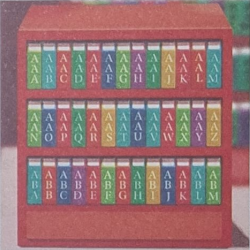
\includegraphics[width=1\linewidth]{imagens_8FMA78/imagem1}
		    \begin{enumerate}[a)]
		    	\item 676
		    	\item 1352
		    	\item 2016
		    	\item 2028
		    	\item 2030\\\\\\\\\\\\\\\\\\\\
		    \end{enumerate}
	        \item Num ginásio de esportes há 7 portas de entrada. De quantas formas podem estar abertas as portas? \\\\\\\\\\\\\\\\\\\\\\\\
	        \item Ao comprar um ingresso para uma peça de teatro, Amanda escolheu uma fileira com oito poltronas para ela e seus sete amigos. Se, no dia da peça, Amanda e Carla não quiserem se sentar lado a lado, de quantos modos os amigos podem ocupar esses lugares? \\\\\\\\\\\\\\\\\\\\\\\\\\\\\\
	        \item Os números de telefone residenciais de uma cidade são formados por 8 dígitos, e o primeiro dígito é diferente de zero. Se os números de telefones residenciais passarem a ter 9 dígitos, ainda com o primeiro dígito diferente de zero, qual será o aumento possível na quantidade de telefones?
        \end{enumerate}
    $~$ \\ $~$ \\ $~$ \\ $~$ \\ $~$ \\ $~$ \\ $~$ \\ $~$ \\ $~$ \\ $~$ \\ $~$ \\ $~$ \\ $~$ \\ $~$ \\ $~$ \\ $~$ \\ $~$ \\ $~$ \\ $~$ \\ $~$ \\ $~$ \\ $~$ \\ $~$ \\ $~$ \\ $~$ \\ $~$ \\ $~$ \\ $~$ \\ $~$ \\ $~$ \\ $~$
    \end{multicols}
\end{document}